\chapter{Mechanical Design}

This chapter includes the mechanical details of Piranha. To begin with, Piranha is a twin-body pontoon boat. It has two floats on the left and right sides to support its weight. The only motorized parts on Piranha are the left and right thrusters installed at the rear. In other words, Piranha is a skid steering boat. Both thrusters provide the driving forces forward or backward, allowing Piranha to move forward and back. The difference between the thruster outputs generates the torque required for steering.

Readers can find The overall design of Piranha in Figure \ref{fig:02rendered_all}.

\begin{figure}[H]
    \centering
    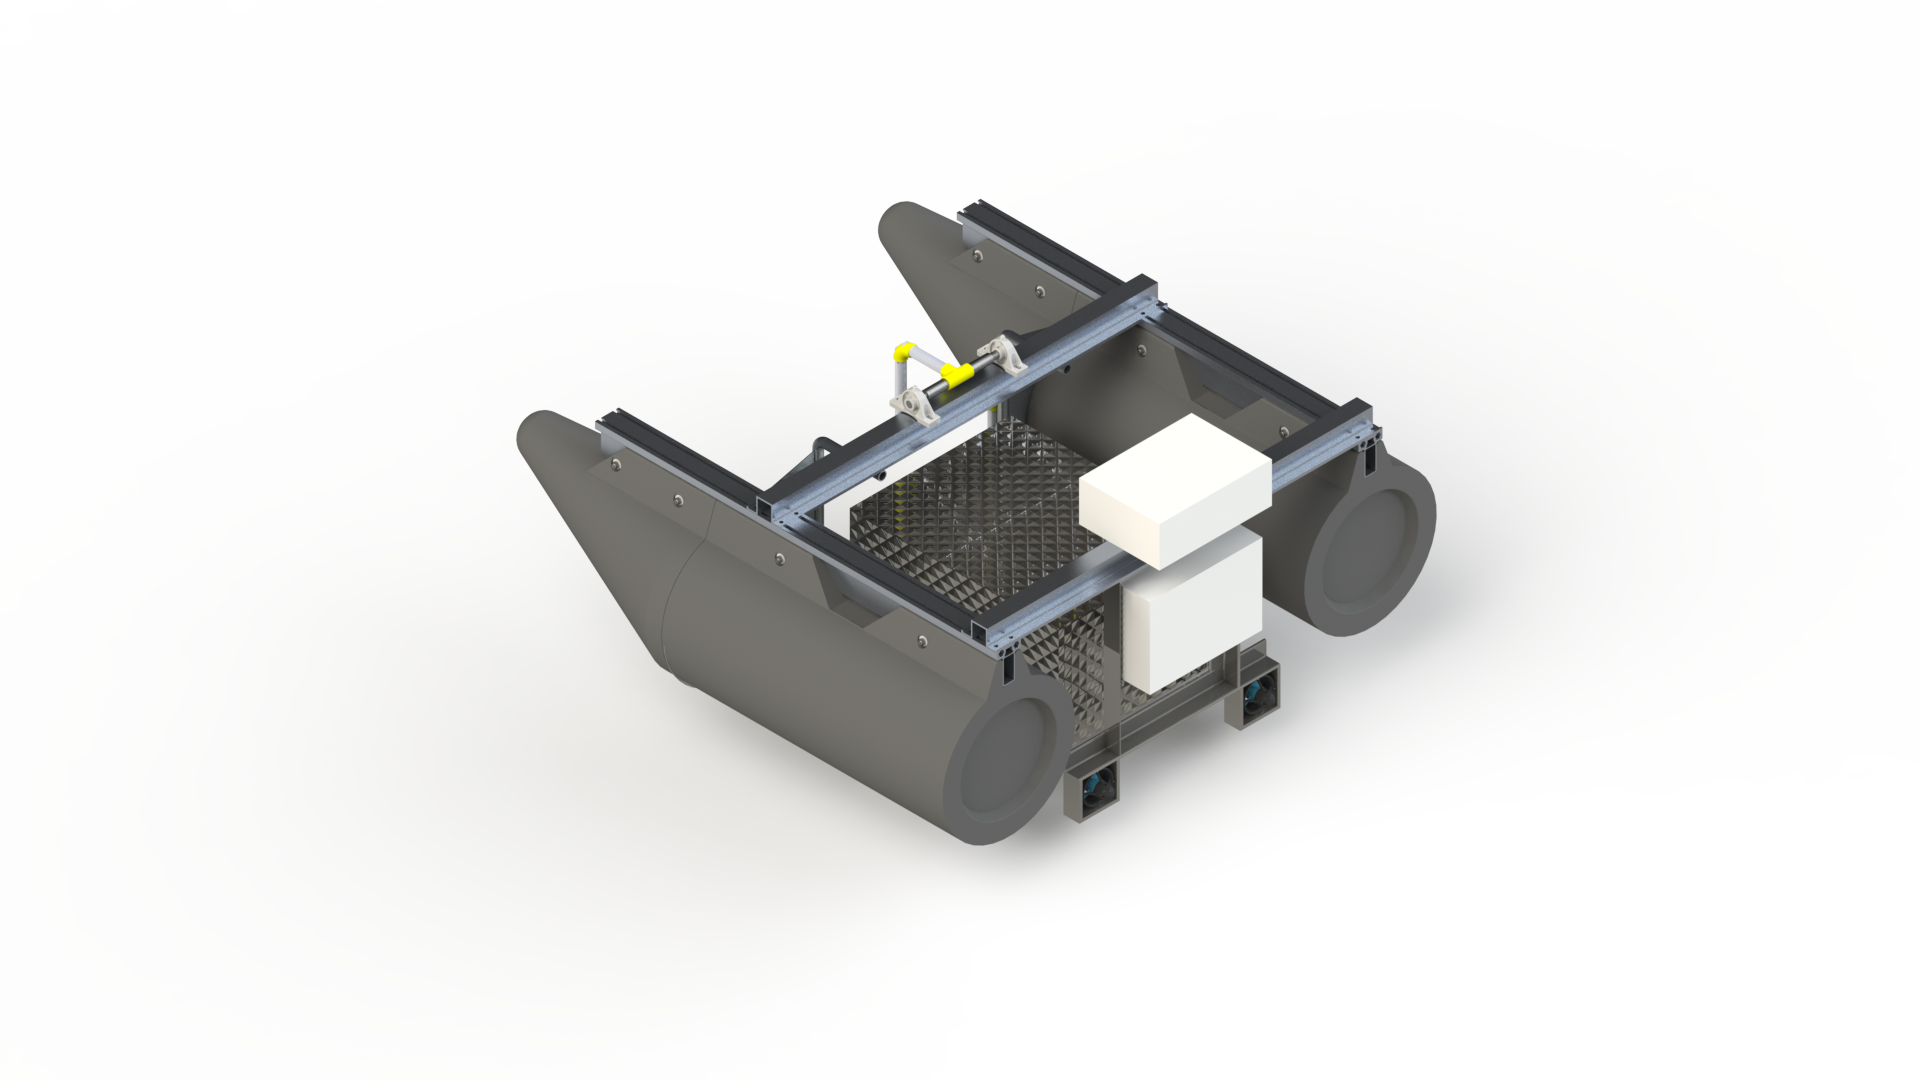
\includegraphics[width=.8\textwidth]{images/02orca-back.png}
    \caption{A rendered model of Piranha. The white blocks represent the electrical system box and the battery pack.}
    \label{fig:02rendered_all}
\end{figure}

\section{Floats}

Piranha's floating parts, including the connection frame, are sold by \textit{Silver Lake Fabrication LLC D.B.A Tiny Pontoon Boats}. The floats are made of High-Density Poly Ethylene (HDPE) with closed-cell urethane foam filling. The connection frame is made of aluminum.

The specifications of the pontoon nose part in Figure \ref{fig:02nose-cone}, can be found in Table \ref{table:02nose-cone}.

\begin{figure}[H]
    \centering
    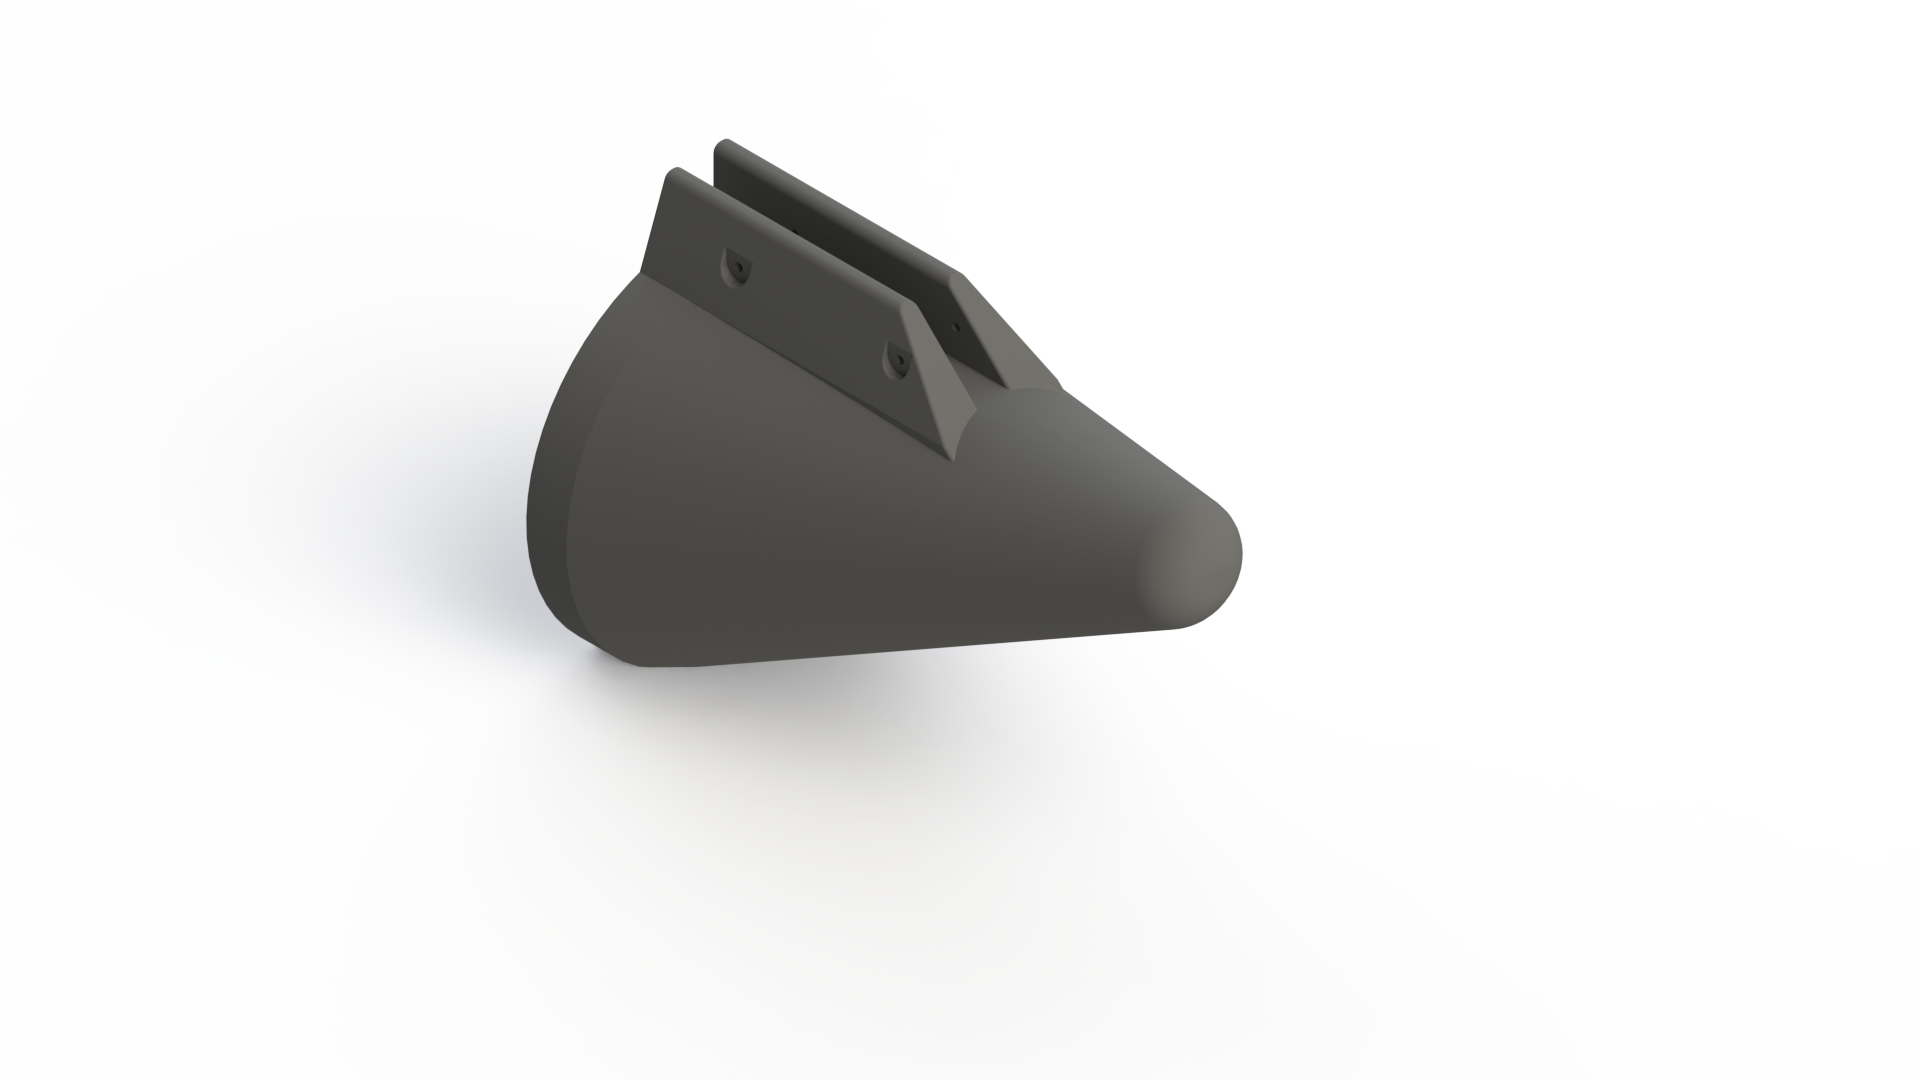
\includegraphics[width=.6\textwidth]{images/02nose-cone.png}
    \caption{Pontoon nose cone.}
    \label{fig:02nose-cone}
\end{figure}

\begin{table}[H]
\caption{Specifications of 17" Diameter Pontoon Nose Cones} % title of Table
\centering % used for centering table
\renewcommand{\arraystretch}{0.8}
\begin{tabular}{l l}
\hline
\textbf{Characteristics} & \textbf{Rating} \\ 
%heading
\hline % inserts single horizontal line
Float width & 16.5 inches \\
Float length & 25 inches \\
Weight & 14 lbs \\
Rated capacity & 45 lbs \\
\hline
\end{tabular}
\label{table:02nose-cone} % is used to refer this table in the text
\end{table}

The specifications of the pontoon straight part in Figure \ref{fig:02pontoon-body}, can be found in Table \ref{table:02pontoon-body}.

\begin{figure}[H]
    \centering
    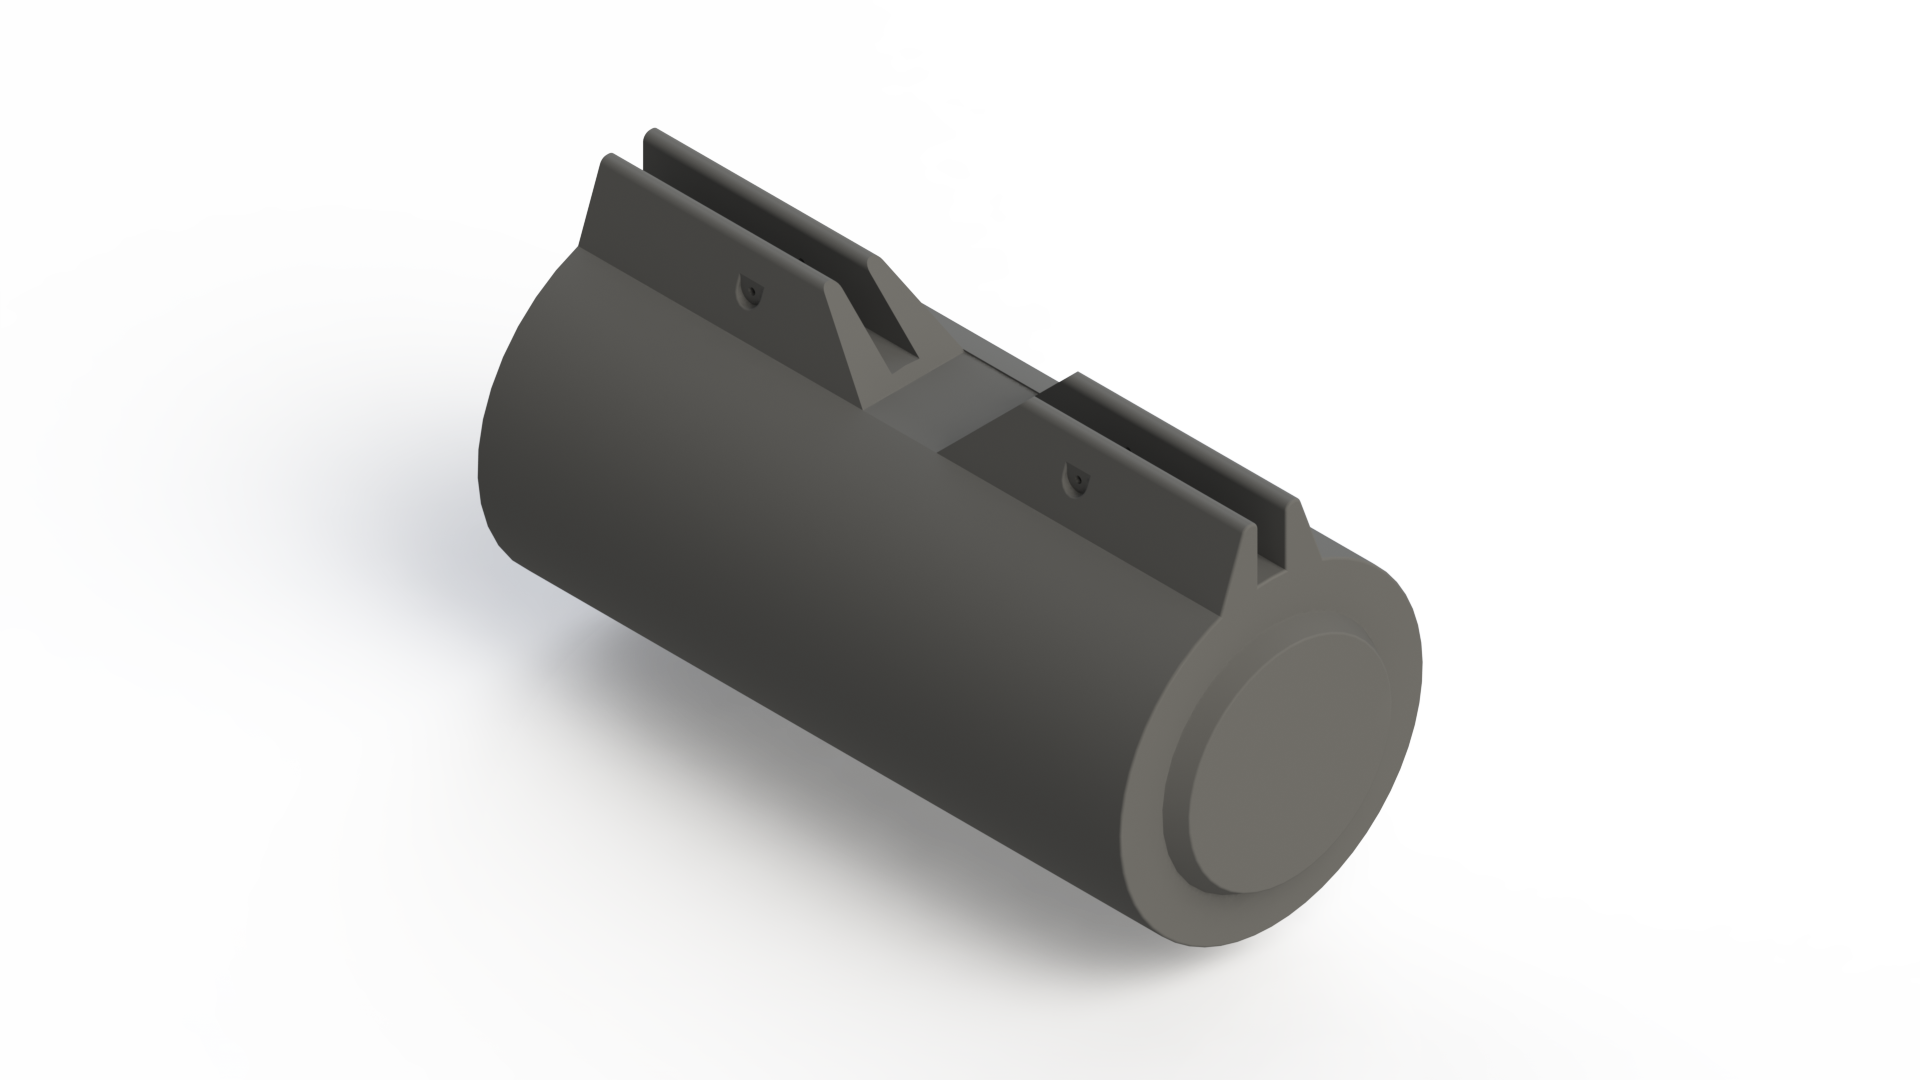
\includegraphics[width=.8\textwidth]{images/02pontoon-body.png}
    \caption{Pontoon body.}
    \label{fig:02pontoon-body}
\end{figure}

\begin{table}[H]
\caption{Specifications of 17" Diameter Pontoon Nose Cones} % title of Table
\centering % used for centering table
\renewcommand{\arraystretch}{0.8}
\begin{tabular}{l l}
\hline
\textbf{Characteristics} & \textbf{Rating} \\ 
%heading
\hline % inserts single horizontal line
Float width & 16.5 inches \\
Float length & 36 inches \\
Weight & 23 lbs \\
Rated capacity & 130 lbs \\
\hline
\end{tabular}
\label{table:02pontoon-body} % is used to refer this table in the text
\end{table}

\subsection{Float Assembly}

Piranha connects the float parts by the aluminum frame, shown in Figure \ref{fig:02orca-frame}. The screws and nuts are made of stainless steel to prevent corrosion.

\begin{figure}[H]
    \centering
    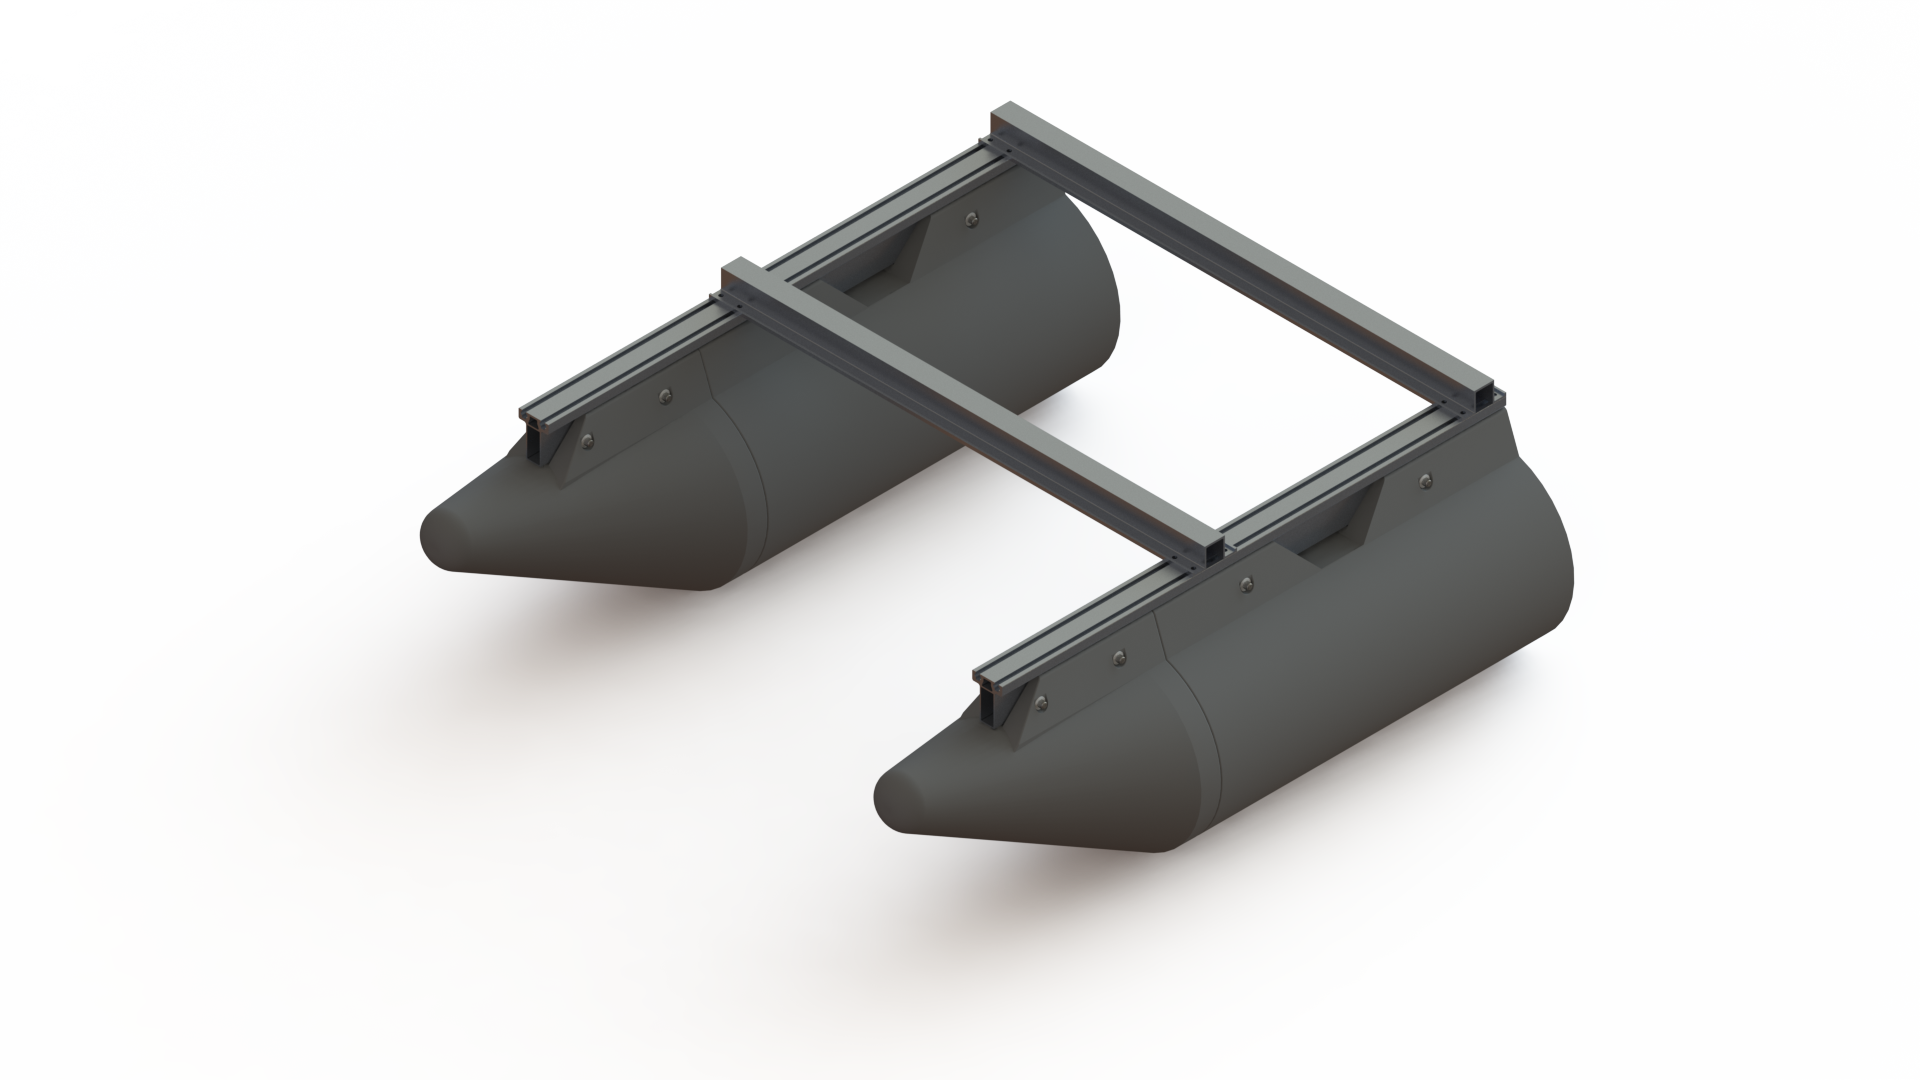
\includegraphics[width=.8\textwidth]{images/02orca-frame.png}
    \caption{The overall float assembly.}
    \label{fig:02orca-frame}
\end{figure}

\section{Thrusters}

Piranha has two thrusters installed at the rear. The thruster model is BlueRobotics T200 Thruster. Its mechanical drawing can be found in Figure \ref{fig:02t200-3d}, \ref{fig:02t200-back}. Table \ref{table:02thruster} lists the specifications for them.

\begin{table}[H]
\caption{Physical Specifications of the BlueRobotics T200 Thruster} % title of Table
\centering % used for centering table
\renewcommand{\arraystretch}{0.8}
\begin{tabular}{l l}
\hline
\textbf{Characteristics} & \textbf{Rating} \\ 
%heading
\hline % inserts single horizontal line
Width & 113 mm \\
Length & 100 mm \\
Weight & 344 g \\
Propeller Diameter & 76 mm \\
\hline
\end{tabular}
\label{table:02thruster} % is used to refer this table in the text
\end{table}

\begin{figure}[H]
    \centering
    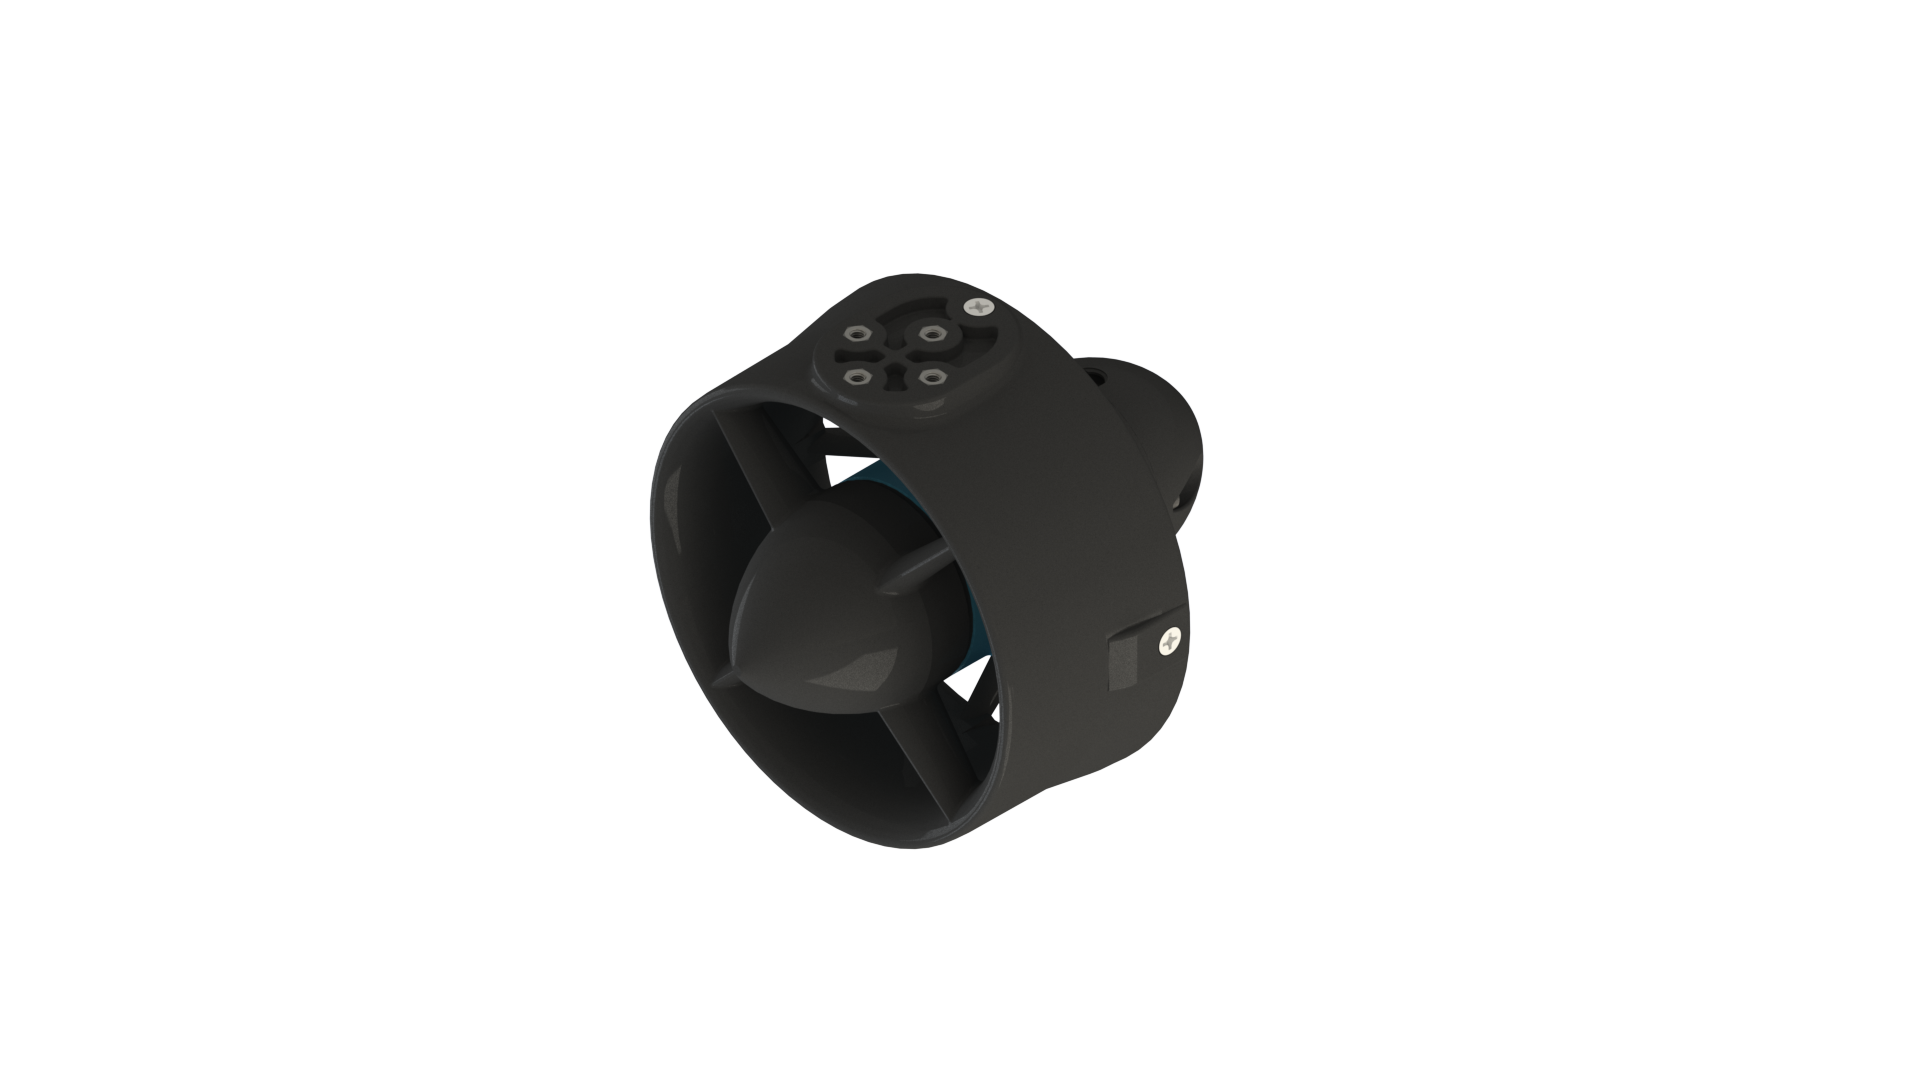
\includegraphics[width=.8\textwidth]{images/02t200-thruster.png}
    \caption{BlueRobotics T200 Thruster (Isometric View).}
    \label{fig:02t200-3d}
\end{figure}

\begin{figure}[H]
    \centering
    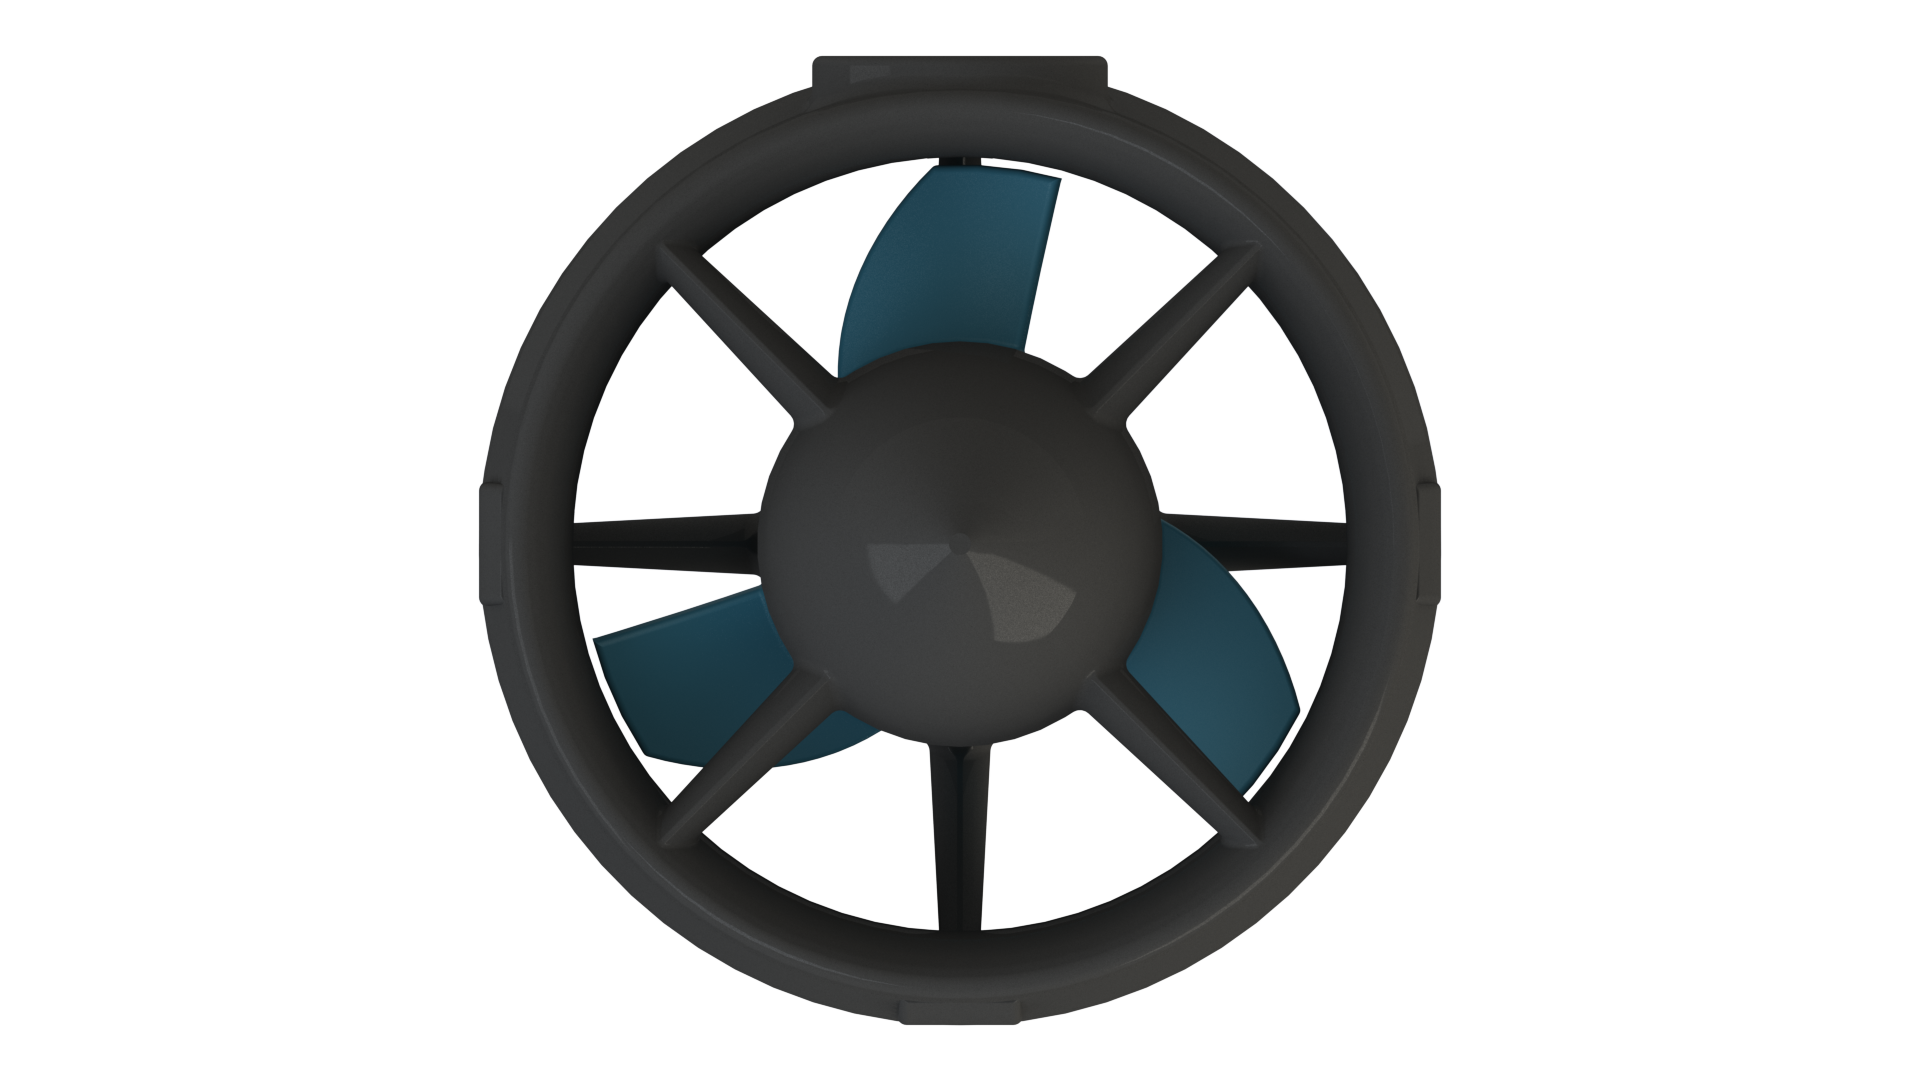
\includegraphics[width=.8\textwidth]{images/02t200-thruster-back.png}
    \caption{BlueRobotics T200 Thruster (Back View).}
    \label{fig:02t200-back}
\end{figure}

\subsection{Thruster Locations}

Figure \ref{fig:02orca-thruster} shows the location of the two thrusters.

\begin{figure}[H]
    \centering
    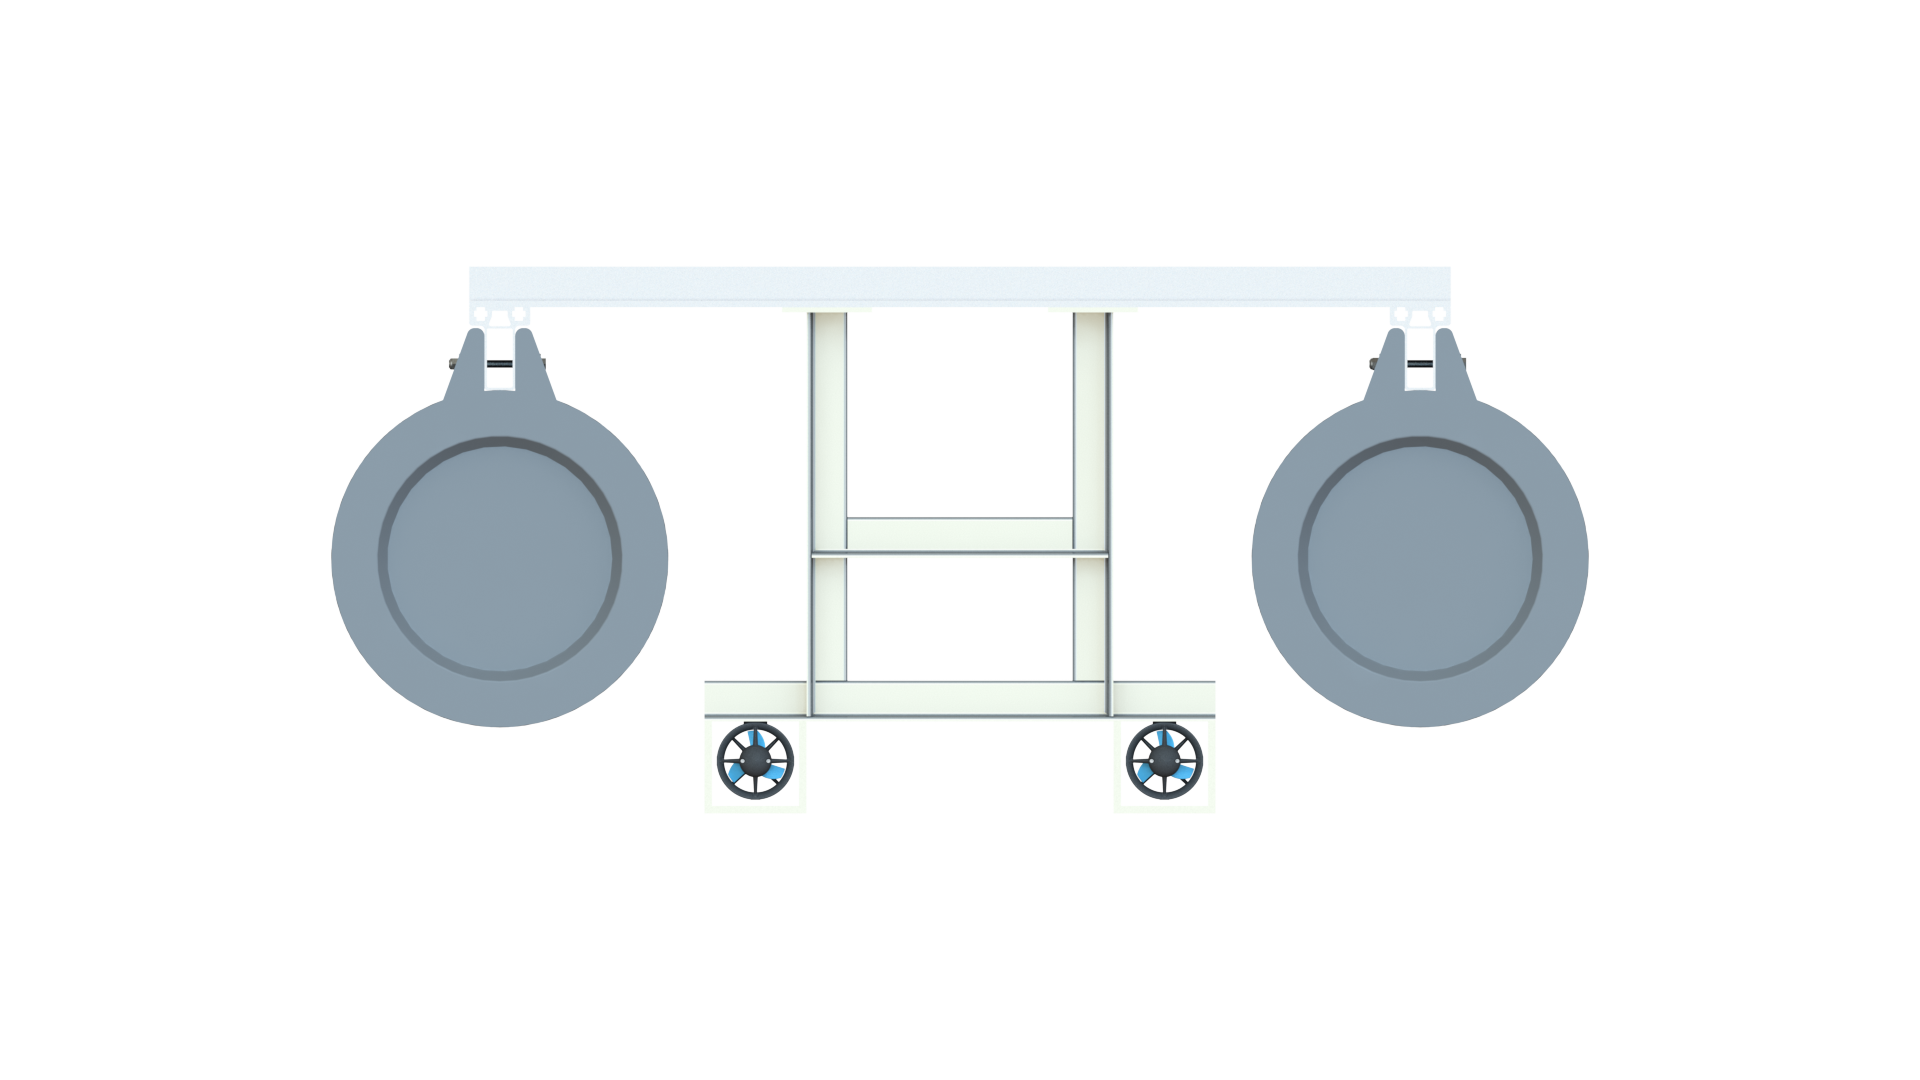
\includegraphics[width=.8\textwidth]{images/02orca-thruster.png}
    \caption{Two thrusters are installed at the rear of Piranha.}
    \label{fig:02orca-thruster}
\end{figure}